\documentclass[../../main.tex]{subfiles}

\begin{document}

Las Redes Neuronales Artificiales (RNAs) son un modelo específico dentro del ML, cuya
estructura y funcionamiento estuvieron inspirados inicialmente por el intento de ser
modelos computacionales del aprendizaje biológico, es decir modelos de cómo el aprendizaje
podría ocurrir en el cerebro \cite{deep-learning}. Durante los últimos años, ha sido el
área que más desarrollo e impacto ha tenido, principalmente gracias a su versatilidad,
potencia y escalabilidad, cualidades que hacen que sean capaces de enfrentar problemas
grandes y complejos \cite{hands-on-ML-sklearn-tf} que hasta el momento parecían
extremadamente difíciles de resolver, como son el reconocimiento de voz y la detección de
objetos.

% Incluirlo?
\subsection{Breve Contexto Histórico}
Aunque su gran éxito ha sido reciente, lo cierto es que la idea de las RNAs data desde
1943, cuando Warren McCulloch y Walter Pitts presentaron en su artículo \textit{A Logical
Calculus of Ideas Immanent of Nervous Activity} \cite{mculloch-pitts-1943} un modelo
computacional simplificado utilizando lógica proposicional acerca de cómo funcionan las
neuronas de cerebros animales en conjunto para llevar a cabo cómputos complejos
\cite{hands-on-ML-sklearn-tf}. Presentaron una versión muy simplificada de la neurona
biológica, que solamente tenía una o más entradas binarias y una salida binaria.

Posteriormente, en 1958, Frank Rosenblatt presentó una de las arquitecturas más simples de
RNAs: el ``Perceptrón'' \cite{rosenblatt1958perceptron}, el cual servía principalmente
para resolver problemas de clasificación en donde los datos son linealmente separables. Su
aporte más notorio es que definió un algoritmo para el entrenamiento del Perceptrón que le
permitía mejorar automáticamente sus parámetros internos para poder llegar a una solución.

Más tarde, se descubrió que los problemas que no podían ser resueltos por el Perceptrón,
sí podían ser resueltos ``apilando'' múltiples perceptrones, lo cual llevó a la invención
del ``Perceptrón Multicapa'' (PMC), también conocido como ``Red Neuronal de Propagación
Directa'' (del inglés \textit{Feedforward Neural Networks}, FFNN) \cite{deep-learning} que
conforman el punto de partida de las redes neuronales actuales.

Para explicar la idea y los elementos presentes detrás de estos algoritmos, tomaremos como
referencia las redes neuronales Feedforward, y en particular las totalmente conectadas,
que definiremos a continuación. Cabe aclarar que las redes neuronales en general se
enmarcan dentro del área del ML conocida como \textbf{Aprendizaje Profundo}.

\subsection{Red Neuronal Feedforward}
Como dijimos anteriormente, las redes neuronales son un modelo particular de Aprendizaje
Automático en el cual las funciones hipótesis toman la forma de circuitos algebraicos
complejos con conexiones que pueden tener diferentes ``intensidades''
\cite{ai-a-modern-approach}. La idea principal en estos circuitos es que el ``camino''
recorrido al realizar el cómputo tenga varios pasos como para permitir que las variables
de entrada puedan interactuar de formas complejas. Esto hace que sean lo suficientemente
expresivos como para poder capturar la complejidad de los datos del mundo real
\cite{ai-a-modern-approach}.

Más concretamente, estos modelos son llamados \textit{redes} porque el espacio de
funciones que proveen está formado en realidad por la composición de varias funciones
\cite{deep-learning}. Por ejemplo, podríamos tener la composición de tres funciones
\(f^{(1)}\), \(f^{(2)}\) y \(f^{(3)}\) para formar la siguiente función:
\begin{equation}
    f(\mathbf{x}) = f^{(3)}(f^{(2)}(f^{(1)}(\mathbf{x})))
    \label{eq:fun-composition}
\end{equation}
donde \(\mathbf{x}\) es un vector de dimensión \(m\) de números reales: \(\mathbf{x}=(x_1,
x_2, ..., x_m)\), es decir \(\mathbf{x} \in \mathbb{R}^m\).

Usualmente, se dice que las redes están organizadas en \textbf{capas}. De esta forma, en
la ecuación anterior, a la función \(f^{(1)}\), que es la primera que se aplica, se la
llama \textbf{capa de entrada}, a \(f^{(2)}\) \textbf{capa oculta o intermedia}, y a
\(f^{(3)}\), que es la que produce el resultado final, \textbf{capa de salida}. La
longitud de esta cadena de funciones es la que va a dar la \textbf{profundidad} de la red.
En general, las RNAs tienen una capa de entrada y una de salida, pero puede tener una o
más ocultas. Cuando tienen una capa oculta, se las llama ``superficiales'' (o poco
profundas, del inglés \textit{shallow}), y cuando tienen más de una \textit{profundas}.

Lo interesante de estos modelos es que si bien el conjunto de entrenamiento especifica qué
tiene que producir la capa de salida ante cada entrada particular, no determina cuál debe
ser el comportamiento de las otras capas \cite{deep-learning}. En cambio, es el algoritmo
de aprendizaje el que tiene que decidir cómo usarlas para lograr una buena aproximación de
la función desconocida.

Una forma muy común y más intuitiva de pensar estos modelos es a través de grafos
dirigidos que describen cómo están compuestas las funciones y cómo fluye la información a
través de ellas. Por ejemplo, la Ecuación \ref{eq:fun-composition} se representaría de la
siguiente manera:
\begin{center}
    \begin{tikzpicture}[
        node distance=2cm,
        every node/.style={draw, circle, minimum size=1cm, align=center},
        thickborder/.style={draw, circle, minimum size=1cm, align=center, line width=0.5mm}
    ]
        % Nodes
        \node (n1) [thickborder] {\( f^{(1)} \)};
        \node (n2) [thickborder, right=of n1] {\( f^{(2)} \)};
        \node (n3) [thickborder, right=of n2] {\( f^{(3)} \)};

        \node (x) [left=of n1 ] {\(\mathbf{x}\)};
        \node (y) [right=of n3] {\( y \)};

        % Edges
        \draw [very thick, ->] (x.east) -- (n1.west);
        \draw [very thick, ->] (n1.east) -- (n2.west);
        \draw [very thick, ->] (n2.east) -- (n3.west);
        \draw [very thick, ->] (n3.east) -- (y.west);
    \end{tikzpicture}
\end{center}

La dirección de las flechas indica el flujo de la información. En este caso, la entrada
\(\mathbf{x}\) va a la función \(f^{(1)}\), la salida de \(f^{(1)}(\mathbf{x})\) va a
\(f^{(2)}\), y la salida de \(f^{(2)}(f^{(1)}(\mathbf{x}))\) va directamente a \(f^{(3)}\)
para de esa forma producir el resultado final \(y = f(\mathbf{x}) =
f^{(3)}(f^{(2)}(f^{(1)}(\mathbf{x})))\). Si hay una flecha que une a dos nodos, diremos
que están ``conectados''.

Es justamente el comportamiento anterior el que caracteriza a las redes neuronales de tipo
\textbf{\textit{feedforward}}: los datos y resultados fluyen en una sola dirección; cada
nodo computa su resultado y se lo pasa a su sucesor (o sucesores, como veremos más
adelante). En el grafo, esta situación se refleja en el hecho que no hay ciclos, por lo
que las redes de este tipo se representan por medio de grafos dirigidos y acíclicos.

Ahora bien, ¿qué es exactamente una capa? En la terminología de redes neuronales, una capa
es un conjunto de \textbf{unidades} o, tomando en cuenta su inspiración biológica,
\textbf{neuronas}, que actúan en paralelo. Cada unidad representa una función que toma un
vector y retorna un escalar, y se asemejan a las neuronas biológicas en el sentido que
reciben entradas (o estímulos) de otras unidades y computan su propio valor de activación
\cite{deep-learning}. De esta forma, las capas se pueden ver como funciones que toman un
vector de vectores y devuelven un vector de escalares.

Cabe aclarar que la capa de entrada va a tener tantas neuronas como la dimensión de los
datos de entrada (\(\mathbf{x}\)). Es decir, si \(\mathbf{x}\) es de dimensión \(m\),
entonces la capa de entrada va a tener \(m\) unidades. Sin embargo, la cantidad de
neuronas de cada capa oculta depende del diseño de la red, y la de la capa de salida
depende sobre todo del problema que se esté tratando de resolver.

Teniendo el concepto de neuronas, podemos introducir el de redes \textbf{totalmente
conectadas} (\textit{fully connected}), que son aquellas en las que cada unidad de una
capa se conecta con todas las de la capa siguiente.

Con esto en mente, podemos concretizar un poco más el ejemplo con el que venimos
trabajando suponiendo que \(\mathbf{x}\) es un vector de dimensión 3, la capa oculta dada
por \(f^{(2)}\) tiene 2 neuronas y la capa de salida tiene 1. Así, suponiendo que nuestra
red es fully connected, nuestro grafo resultaría en:
\begin{center}
    \begin{tikzpicture}[
        node distance=1.5cm,
        every node/.style={draw, circle, minimum size=1cm, align=center},
        connect arrow/.style={-{Latex[length=4,width=3.5]}, very thick, mydarkblue,
        shorten <=1,shorten >=1},
    ]
        % Inputs
        \node (x1) {\(x_1\)};
        \node (x2) [below=of x1] {\(x_2\)};
        \node (x3) [below=of x2] {\(x_3\)};

        % Input layer
        \node (f11) [right=of x1] {\(f^{(1)}_1\)};
        \node (f12) [right=of x2] {\(f^{(1)}_2\)};
        \node (f13) [right=of x3] {\(f^{(1)}_3\)};

        % Hidden layer
        \node (f21) [right=of $(f11)!0.5!(f12)$] {\(f^{(2)}_1\)};
        \node (f22) [below=of f21] {\(f^{(2)}_2\)};

        % Output layer
        \node (f31) [right=of $(f21)!0.5!(f22)$] {\(f^{(3)}_0\)};

        % Output
        \node (y) [right=of f31] {\( y \)};

        % Edges
        \draw [connect arrow] (x1.east) -- (f11.west);
        \draw [connect arrow] (x2.east) -- (f12.west);
        \draw [connect arrow] (x3.east) -- (f13.west);

        \draw [connect arrow] (f11.east) -- (f21.west);
        \draw [connect arrow] (f12.east) -- (f21.west);
        \draw [connect arrow] (f13.east) -- (f21.west);
        \draw [connect arrow] (f11.east) -- (f22.west);
        \draw [connect arrow] (f12.east) -- (f22.west);
        \draw [connect arrow] (f13.east) -- (f22.west);

        \draw [connect arrow] (f21.east) -- (f31.west);
        \draw [connect arrow] (f22.east) -- (f31.west);

        \draw [connect arrow] (f31.east) -- (y.west);
    \end{tikzpicture}
\end{center}
donde el subíndice de cada nodo hace referencia al número de neurona en esa capa.

Vemos entonces cada neurona de la capa de entrada se encarga de recibir una ``parte'' del
vector de entrada, pero las neuronas de tanto la capa oculta como la de salida reciben las
salidas de las neuronas de la capa anterior. Veamos entonces qué hace precisamente una
neurona o unidad.

Una neurona simplemente calcula una suma pesada de sus entradas, provenientes de las
unidades de la capa anterior, y luego aplica una función \textbf{no lineal} que
denotaremos con \(a\) para producir su salida. Formalmente, si denotamos con \(s^{(k)}_j\)
la salida de la unidad \(j\) de la capa \(k\), \(a^{(k)}_j\) la función no lineal de la
unidad, y con \(w_{i,j}\) la intensidad o \textbf{peso} de la conexión entre una neurona
\(i\) de la capa anterior y la \(j\) de la capa actual, tenemos que:
\begin{equation}
    s^{(k)}_j = a^{(k)}_j \left( \sum_i w_{i,j} s^{(k-1)}_i \right) = a^{(k)}_j (in^{(k)}_j)
    \label{eq:neuron}
\end{equation}

Si en nuestro ejemplo tomamos la neurona \(f^{(2)}_1\), tenemos que su salida estará dada
por:
\begin{align*}
    s^{(2)}_1 &= a^{(2)}_1 \left( \sum_{i=1}^{3} w_{i,1} s^{(1)}_i \right) \\
              &= a^{(2)}_1 \left( w_{1,1}s^{(1)}_1 +  w_{2,1}s^{(1)}_2 + w_{3,1}s^{(1)}_3 \right)
\end{align*}

En las redes, se estipula que cada unidad tiene una entrada extra desde una neurona
\textit{dummy} de la capa anterior, para la cual utilizaremos el subíndice 0, cuyo valor
está fijado en 1 y su peso correspondiente será \(w_{0,j}\) para una capa \(j\). Esto
permite que el valor \(in^{(k)}_j\) sea distinto de 0 incluso cuando todas las salidas de
la capa anterior sean 0 \cite{ai-a-modern-approach}. Este término nos permite escribir la
Ecuación \ref{eq:neuron} de forma vectorizada:
\begin{equation}
    s^{(k)}_j = a^{(k)}_j \left( \mathbf{W}^T \mathbf{x} \right)
\end{equation}
donde \(\mathbf{W}\) es el vector de todos los pesos que se dirigen a la unidad \(j\) de
la capa \(k\) (incluyendo \(w_{0,j}\) y \(\mathbf{x}\) es el vector de todas las entradas
de la unidad \(j\) de la capa \(k\) (incluyendo el 1 fijo de la neurona dummy).

Si tomamos nuevamente a \(f^{(2)}_1\), tenemos:
\begin{quote}
    \(\mathbf{W} = (w_{0,1}, w_{1,1}, w_{2,1}, w_{3,1})\),
    \(\mathbf{X} = (1, s^{(1)}_1, s^{(1)}_2, s^{(1)}_3)\)
\end{quote}

La función \(a^{(k)}_j\) se denomina \textbf{función de activación}, y el hecho que sea no
lineal es importante ya que de no ser así, cualquier composición de unidades estaría
representando una función lineal \cite{ai-a-modern-approach}. Es justamente esta no
linealidad lo que permite a estos modelos representar funciones arbitrarias
\cite{ai-a-modern-approach}.

Algunas funciones de activación comunes son las siguientes:
\begin{itemize}
    \item \textbf{Sigmoide}: \(\sigma(x)=\frac{1}{1+e^{-x}}\)
    \item \textbf{ReLU} (abreviatura de \textit{rectified linear unit}):
    \(\text{ReLU}(x) = \text{max}(0, x)\)
    \item \textbf{Tangente hiperbólica}: \(\text{tanh}(x)=\frac{e^x - e^{-x}}{e^x + e^{-x}}\)
\end{itemize}
Actualmente, la más utilizada es la ReLU y variantes de ella.



% EScribir la composición final



\subsubsection{Entrenamiento}

% Función de costo: back-propagation
% Optimizador
% Hiperparámetros: conjunto de validación, cross-validation
% Pesos
% Otras optimizaciones: lotes, detención temprana, dropout

\begin{comment}
Esto se puede ver gráficamente en la Figura \ref{fig:neuron}.

\begin{figure}[h!]
    \centering
    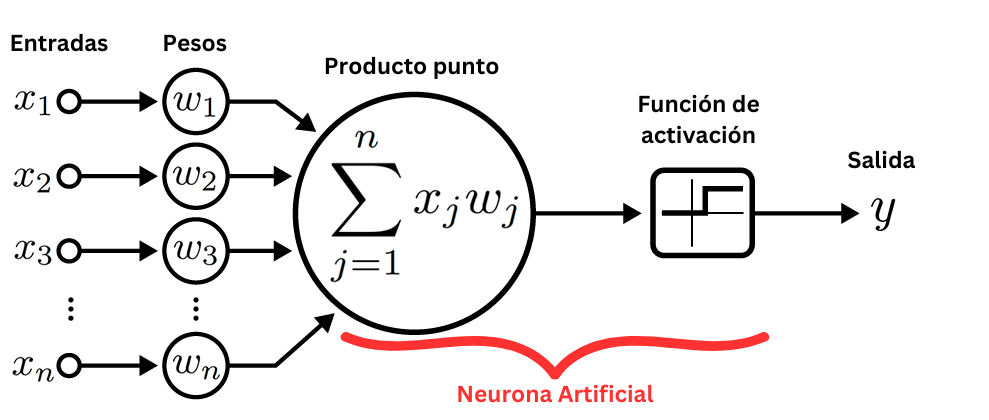
\includegraphics[width=0.6\textwidth]{figs/neurona.png}
    \caption{La neurona computa una suma pesada de sus entradas y aplica una función
    de activación sobre el resultado.}
    \label{fig:neuron}
\end{figure}

La idea detrás de la función de activación es el hecho de propagar la información
proporcionalmente al estímulo provocado por las entradas en la neurona, basándose en la
idea de ``disparo'' de una neurona biológica en el momento en que se supera el umbral de
activación. La función de activación utilizada en el Perceptrón, mencionado anteriormente,
fue la llamada \textit{heavyside}, dada por:
\[
    heavyside\left(z\right) =
        \begin{cases}
            0\text{ si }z < 0 \\
            1\text{ si }z \geq 0
        \end{cases}
\]

Durante los años, se han empleado diferentes funciones de activación, como la sigmoide, la
tangente hiperbólica, y la ReLU, dada por \(\text{ReLU}(z)=\text{max}(0, z)\), siendo esta
última la más común actualmente.

Dicho esto, en una red neuronal está compuesta por diferentes \textbf{capas de neuronas}:
la capa de entrada, que es por donde ingresan los datos, una o más capas ocultas o
intermedias, y finalmente la capa de salida.

\begin{figure}[h!]
    \centering
    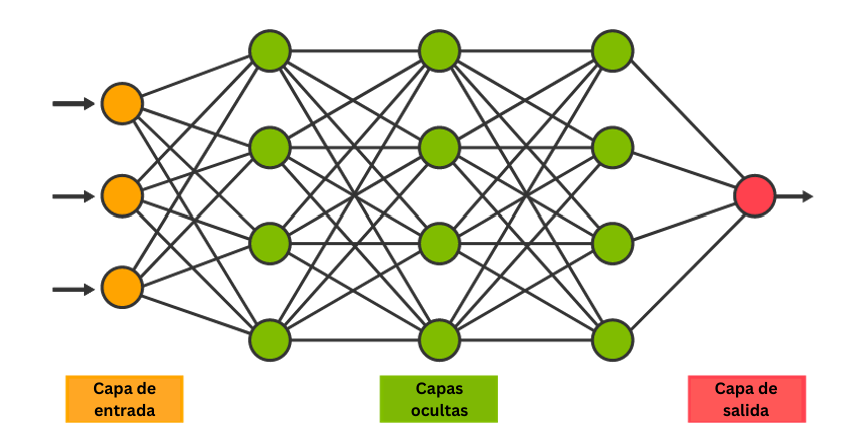
\includegraphics[width=0.6\textwidth]{figs/feedforward.png}
    \caption{Esquema de una Red Neuronal Profunda, con tres capas ocultas. Las neuronas
    naranjas forman la capa de entrada, las neuronas verdes forman las tres capas ocultas,
    y la roja la de salida. Cabe notar que la capa de salida podría tener más de una neurona.}
    \label{fig:neural-net}
\end{figure}

Ahora bien, el objetivo de una red neuronal es \textbf{aproximar una función desconocida}
\(g^*\). Para un clasificador por ejemplo, \(y=g^*(x)\) determina una categoría \(y\) para
una entrada \(x\). De esta forma, una red define una asignación \(y=g(x; \theta)\) y
aprende el valor de los \textbf{parámetros} \(\theta\) que resultan en la mejor
aproximación de la función ``oculta'' \cite{deep-learning}. En este caso, los parámetros a
aprender por la red serán los pesos sinápticos de todas las conexiones.

Matemáticamente, los pesos entre una capa de neuronas y la siguiente se pueden pensar como
una matriz \(w\), en donde la entrada \(w_{ij}\) indica el peso sináptico de la conexión
entre la neurona \(i\) de la capa ``actual'' y la neurona \(j\) de la capa ``anterior''.
La pregunta que surge entonces es \textbf{cómo} hacer para que la red pueda aproximar esta
función.

\subsubsection{Entrenamiento de una RNA Feedforward}
A grandes rasgos, el entrenamiento de una red consiste en una suma de \textbf{evaluación}
y \textbf{optimización} \cite{pedro-domingos}. Con evaluación, nos referimos al
establecimiento de una medida que determine qué tan lejos está el modelo de hallar una
buena solución, para lo cual se suele definir una función a minimizar o maximizar llamada
\textbf{función objetivo} o \textbf{criterio} \cite{deep-learning}; y la optimización es
el método usado para aproximarse a dicha solución, maximizando o minimizando la función
objetivo según corresponda.

Cuando lo deseado es minimizar la función objetivo, esta pasa a ser llamada
\textbf{función de costo}, \textbf{función de error} o \textbf{función de pérdida}. En
problemas de aprendizaje supervisado, esta función compara la salida de la red para
determinadas entradas - la \textbf{predicción} - en su estado actual, dado por el valor de
los pesos sinápticos en ese momento, con las salidas reales para dichas entradas, dadas
por el conjunto de entrenamiento. En resumen, una vez que están fijos los datos del
conjunto de entrenamiento, la función de costo es una función de los pesos de la red. Por
lo tanto, la denotaremos con \(f(w)\).

Dos de las funciones de costo más utilizadas son el \textbf{Error Cuadrático Medio} y la
\textbf{Entropía Cruzada}. De estas dos funciones, nos concentraremos en la última ya que
es la más apropiada para problemas de clasificación como el que tratamos. Esto se debe a
que mide la diferencia entre la distribución de probabilidad predicha por el modelo y la
distribución real de los datos.  En este caso, la capa de salida tiene tantas neuronas
como categorías haya, y la salida de cada una de ellas representa el puntaje que le da la
red a la categoría correspondiente a cada neurona, donde un mayor puntaje indica una mayor
probabilidad de pertenencia de la entrada particular a dicha clase. Para obtener una
estimación de la distribución de probabilidad dada por estas salidas, se aplica la función
\textit{softmax} \cite{hands-on-ML-sklearn-tf}.

Una vez que se tiene esta función establecida y se calculan las pérdidas para los datos,
el algoritmo por defecto que se utiliza para la optimización es el de \textbf{Descenso por
el Gradiente} (\textit{Gradient Descent}). Este se basa en modificar los parámetros (i.e.
los pesos sinápticos) iterativamente con el objetivo de encontrar mínimos locales de una
función, que en este caso será la de costo. Se basa en la idea que la dirección dada por
el gradiente es la de mayor crecimiento, y por lo tanto su opuesta es la de menor. De esta
forma, lo que se hace en cada paso es calcular el gradiente de la función de costo con
respecto a los pesos, y luego actualizarlos siguiendo la siguiente regla:
\[
w = w - \eta \ \nabla f(w),
\]
donde \(w\) representa una matriz de pesos de una determinada capa, y la cantidad \(\eta\)
es llamada la \textbf{tasa de aprendizaje}, que determina el tamaño de cada paso. Si
\(\eta\) es muy pequeño, entonces el algoritmo tendrá que hacer muchos pasos para
converger; pero si es demasiado grande, puede llegar a divergir.

Actualmente, se utilizan otros optimizadores más sofisticados y eficientes, pero que todos
parten de la idea del Descenso por el Gradiente. Los que usaremos en los experimentos son
el Descenso por el Gradiente Estocástico (\textit{Stochastic Gradient Descent}, SGD) y
Adam (\textit{Adaptive Moment Estimation}), de los cuales se puede leer más en el Capítulo
8 de \cite{deep-learning}.

Ahora bien, recordando que la función \(f\) está fija en todas las entradas y salidas del
conjunto de entrenamiento, hay algoritmos de optimización que utilizan todos estos datos
para  calcular el gradiente, otros que utilizan de a un ejemplo a la vez para calcular el
gradiente y otros que están entre medio de los dos anteriores, es decir utilizan un
subconjunto del conjunto de datos para calcular el gradiente (esto es lo que hace SGD).

Es necesario en este punto introducir el concepto de ``\textbf{época}'' y de
``\textbf{lote}''. Un lote es simplemente una subdivisión de tamaño fijo del conjunto de
entrenamiento (o de test). Dicho esto, se llama época al proceso completo en el cual el
modelo entrena utilizando \textbf{todos} los datos disponibles en el conjunto de
entrenamiento una vez, ya sea recorriéndolos de a lotes o todos de una vez. Si el conjunto
está efectivamente dividido en lotes, una época va a consistir de: \textbf{para cada
lote}, calcular las predicciones en base a los pesos actuales, obtener los errores de cada
muestra del lote, computar los gradientes en base a los ejemplos del lote y actualizar los
pesos. Si no, se hacen los mismos pasos pero para todos los datos de una vez.

Al entrenar un modelo, existen ciertos ajustes que son utilizados para controlar su
comportamiento llamados \textbf{hiperparámetros}. Los valores de los hiperparámetros no
son aprendidos por el modelo \cite{deep-learning}, sino que se fijan de antemano y no se
modifican a lo largo del entrenamiento. Algunos de estos son: la cantidad de neuronas en
cada capa oculta, la función de activación utilizada en cada capa, el optimizador, la tasa
de aprendizaje, el número de épocas, el tamaño de lote, entre otros. Todos estos pueden
contribuir a que el modelo mejore su desempeño. Para probar distintos valores de
hiperparámetros, que es lo que haremos a continuación, se utiliza un conjunto de datos
extra además del de entrenamiento y el de test, llamado de \textbf{validación} que sirve
justamente para encontrar los hiperparámetros óptimos.

% Mejoras extras: detención temprana, dropout
Otras mejoras que se han implementado para mejorar la eficacia de los modelos, y que
emplearemos en los experimentos, son las nombradas a continuación. Por un lado, tenemos la
\textbf{detención temprana}, que consiste en frenar el entrenamiento en el último mejor
``estado'' del modelo cuando se observa que a partir de dicho punto el error sobre el
conjunto de validación no mejora (notar que cuántas épocas se espera y qué se considera
una mejora son nuevos hiperparámetros). Y por otro lado, el \textbf{dropout}, que es un
algoritmo que implica suprimir un cierto número de neuronas de una capa de manera
aleatoria \cite{apuntes-redes-neuronales}.
\end{comment}

\end{document}